\chapter{Platform deployment and demonstrations}\label{H:platformDeploymentAndDemonstrations}

In order to demonstrate that the LiveMediaStreamer is a suitable tool to be used as the core framework of a cloud real-time media production platform it's required to showcase how it performs over the cloud. Therefore, it's important to demonstrate how it performs over the proposed architecture. And, previous chapters have implicitly helped to deploy and demonstrate it as shown in this chapter.

\section{Platform deployment}

In order to demonstrate how LMS suits to become a proper tool it's proposed to deploy two scenarios with different complex degrees.

\begin{itemize}
\item Isolated deployment \hfill

The main goal of this deployment is to demonstrate how LMS performs inside a Docker container by comparing its performance in the same O.S. but without running inside a container (i.e.: system installation).

In this scenario deployment LMS is configured to act as a transcoder service. This means applying one pipeline per stream type (i.e.: one video and one audio paths).

\item Generic scenario deployment \hfill

This scenario deployment aims to showcase a suitable and a as much generic as possible cloud real-time media production scenario. Therefore, it is proposed to configure LMS to receive eight streams (i.e.: four audio and four video streams), mix them and transmit them through RTP/RTSP and MPEG-DASH. 
\end{itemize}

The environment where the deployments are done has the following characteristics:

\begin{table}[htb]
\caption{Deployment environment characteristics}
\begin{center}
\begin{tabular}{|c|c|}
\hline
{\bf Parameter} & {\bf Value} \\ \hline \hline
Hardware type        & Sony Vayo laptop \\ \hline
CPU        & Intel core i7-3632QM at 2.20 GHz  \\ \hline
RAM        & 6 GB (4 + 2) DDR3 \\ \hline
Operating system        & XUbuntu 14.04 - 64 bits (x86 64)  \\ \hline
Kernel version        & 3.13.0-55-generic  \\ \hline
Docker version        & 1.6.8  \\ \hline
\end{tabular}
\label{T:dec}
\end{center}
\end{table}

As seen, the deployment hasn't been carried out in any type of specific server or high performance environment. This is mainly due to demonstrate characteristics such as flexibility on the deployment (i.e.: in a laptop) and portability of the platform (not only the cloud itself). And, all of these characteristics are achieved thanks to the performance of the platform itself and, concretely, the LMS (the core).

\subsection{Isolated demonstrations}

In order to demonstrate results of interest what is done is to implement a C/C++ script which configures the LMS framework as shown in figure \ref{F:idsc}. Moreover, in order to test how it performs the pipeline metrics are logged once per second (i.e.: pipeline losses and delay) and gathered by a Collectd client container properly configured. Then the Collectd client sends the data to the Graphite container. 

\begin{figure}[htb]
\begin{center}
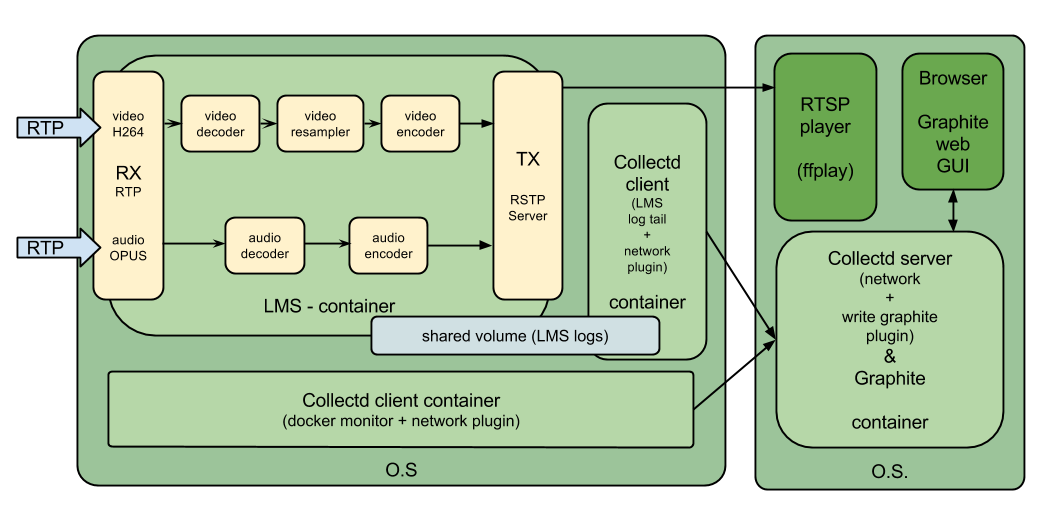
\includegraphics[width=0.95\textwidth]{./images/isolatedScenario.png}
\caption{Isolated demonstration's scenario configuration}
\label{F:idsc}
\end{center}
\end{figure}

The Collectd client container, which reads from the volume where the LMS container is logging its metrics, is using the "tail" plugin (previously explained in chapter \ref{G:monitoringLayer}) with specific regular expressions in order to parse the metrics from the LMS logs (See APPENDIX XXX for this specific collectd configuration)

So, both isolated scenarios are the same but one is running the LMS on the system and the other is running the same configure LMS but containerized.

EXPLICACIÓ ESCENARI (les fonts venen del mateix pc player - un mac amb linux) I 
RESULTATS


\subsection{Generic scenario demonstration}

This last scenario aims to be a generic and basic example demonstration of audio and video production in a cloud environment. Figure \ref{F:gdsc}



\begin{figure}[htb]
\begin{center}
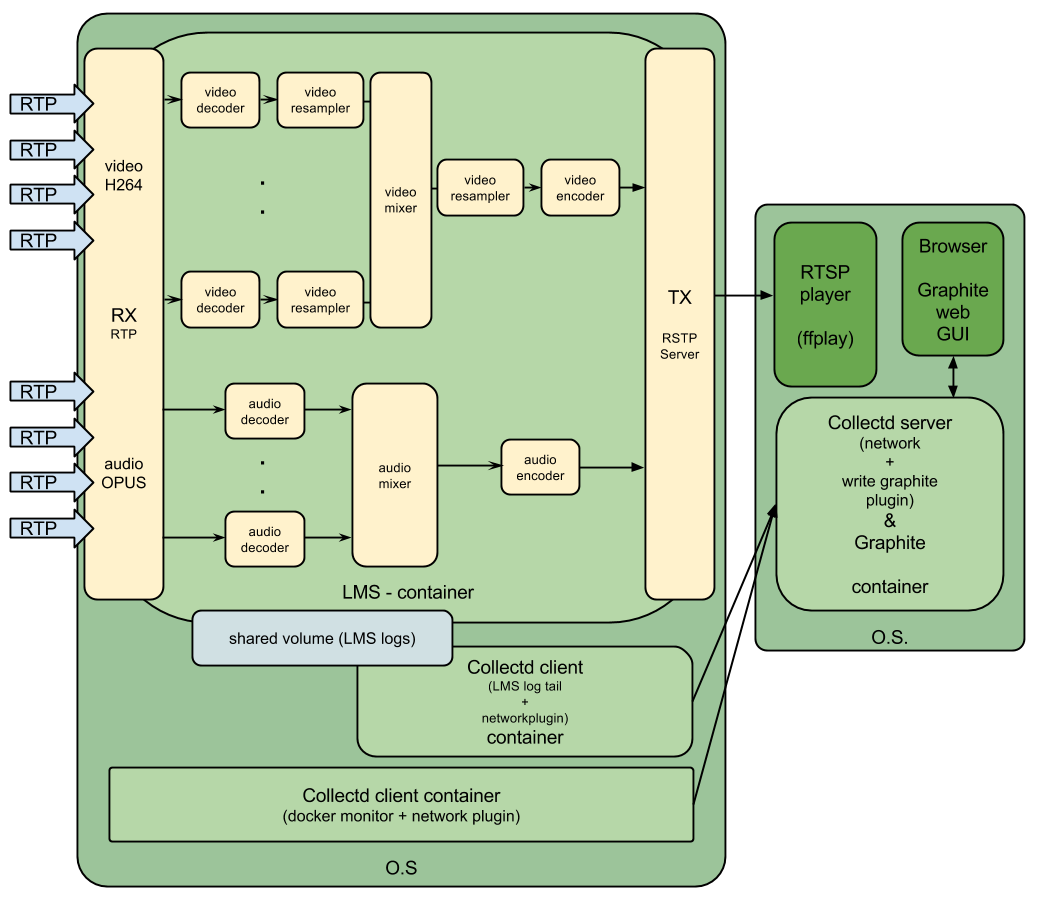
\includegraphics[width=0.95\textwidth]{./images/genericScenario.png}
\caption{Generic demonstration's scenario configuration}
\label{F:gdsc}
\end{center}
\end{figure}